%\part{Einfuehrung} 

%----------------------------------------------------------------------------
\section{Einführung}
\begin{frame}
\frametitle{Einführung}
	\huge Einführung in die Programmierung
\end{frame}

\begin{frame}
\frametitle{Ihre Erwartungen an die Veranstaltung}
	\begin{exampleblock}{Was m\"ochten Sie gerne behandeln?}
		\begin{itemize} 
			 \item{Parallele Programmierung mit Threads}
			 %\item{Netzwerkprogrammierung}
			 \item{}
			 \item{}
			 \item{}
		\end{itemize}
	\end{exampleblock}
\end{frame}
 
\begin{frame}
\frametitle{Erwartungen an die Veranstaltung}
	\begin{block}{Was sollten Sie am Ende k\"onnen?}
		\begin{itemize}
			 \item{Eigenständig einfache Programme schreiben}
			 \item{Anweisungen, Ausdrücke, Operatoren, Kontrollstrukturen und Schleifen
			 kennen}
			 \item{Datentypen, Variablen und Konstanten kennen und sinnvoll einsetzen}
			 \item{Mit Strings und Arrays sicher umgehen}
			 \item{Das Prinzip der Rekursion verstehen und anwenden}
			 \item{Sich selbständig in Java weiterentwickeln}
			 \item{Die vorgestellten Konzepte verstehen und anwenden}
		\end{itemize}
	\end{block}
\end{frame}

\begin{frame}
\frametitle{In der Veranstaltung verwendete Werkzeuge}
	\setbeamerfont{block title}{size=\scriptsize}
	\begin{columns}[T]
	    \begin{column}{.5\textwidth}
	    	\begin{block}{Programmiersprache}
	    		\center
	    		
\includegraphics[width=1\textwidth, keepaspectratio=true]{bilder/java.jpeg}
	    	\end{block}
	    \end{column}
	    \begin{column}{.5\textwidth}
	     	\begin{block}{Entwicklungsumgebung}
	     		\center
	     		
\includegraphics[width=1\textwidth, keepaspectratio=true]{bilder/eclipse.jpg}
	    	\end{block}
	    \end{column}
	\end{columns}
	\setbeamerfont{block title}{size=\normalsize}
\end{frame}
 
\subsection{Programmiersprache}
\begin{frame}
\frametitle{Warum Java?}
	\begin{block}{Java ist\ldots}
 		\begin{itemize}
		  \item Weit verbreitet.
		  \item Verh\"altnism\"a"sig leicht zu erlernen.
		  \item Plattformunabh\"angig.
		  %\item Objektorientiert.
		\end{itemize} 
	\end{block}
	\begin{exampleblock}{Dokumentation}
		\url{http://docs.oracle.com/javase/7/docs/api/}
	\end{exampleblock}
\end{frame}
 
\subsection{Entwicklungsumgebung}
\begin{frame} 
\frametitle{Eclipse erleichtert uns die Entwicklung}
	\begin{columns}
	    \begin{column}{.5\textwidth}
			\small
			\begin{itemize}
			  \item Integrated Development Environment
			  \item Verwaltet Dateien in Projekten
			  \begin{item}
			  		Es existieren 4 Hauptkomponenten:
					\begin{enumerate}
					  \item \tiny Workspaces
					  \item \tiny Projekte (Projects)
					  \item \tiny Perspektiven (Perspectives)
					  \item \tiny Sichten (Views)
					\end{enumerate}
			  \end{item} 
			\end{itemize}
			\normalsize
	    \end{column}
	    \begin{column}{.5\textwidth}
	   		\center
	    	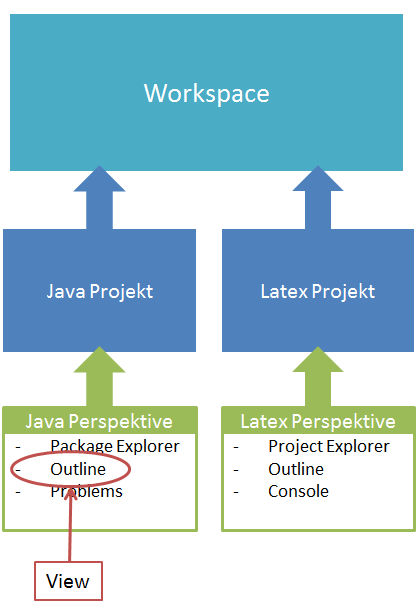
\includegraphics[width=1\textwidth, keepaspectratio=true]{bilder/workspace.png}
	    \end{column}
	\end{columns}
\end{frame}

\subsection{Programmiersprachen}
\begin{frame}[fragile]
	\frametitle{Einordnung der prozeduralen Programmierung}
			Imperative Programmierung
			\small
			\begin{itemize}
			  \item Prozedurale Programmierung\\
			  z.B. C, Cobol, Pascal
			  \item Objektorientierte Programmierung\\
			  z.B. Java, C\#, SmallTalk
			  \item Skriptsprachenorientierte Programmierung\\
			  z.B. PHP, JavaScript, Perl, Python
			\end{itemize}
			\normalsize
	   		\vspace{0.3cm}
	   		Deklarative Programmierung
			\small
			\begin{itemize}
			  \item Funktionale Programmierung\\
			  z.B. Lisp, Haskell
			  \item Prädikative Programmierung\\
			  z.B. Prolog
			\end{itemize}
			\normalsize
\end{frame}

\subsection{John-von-Neumann}
\begin{frame}[fragile]
	\frametitle{John-von-Neumann-Architektur}
	\begin{columns}
	   		\begin{column}{.5\textwidth}
				Gesamtkonzept für den Aufbau eines universellen Rechners.
				\newline\newline
				Besteht aus folgenden Komponenten:
				\begin{itemize}
				  \item Steuerwerk
				  \item Rechenwerk
				  \item Speicher
				  \item Eingabewerk
				  \item Ausgabewerk
				\end{itemize}
				\end{column}
				    	\begin{column}{.5\textwidth}
				   		\center
				    	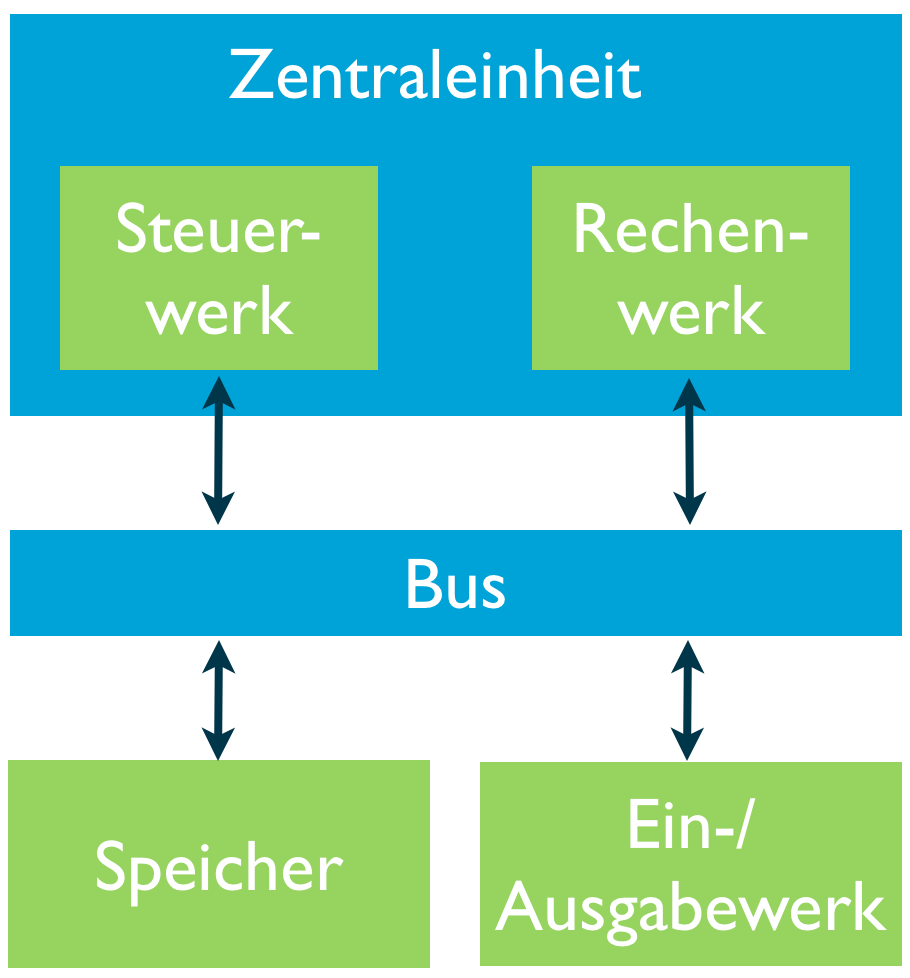
\includegraphics[width=1\textwidth,
				    	keepaspectratio=true]{bilder/universal_rechner.png}
	    \end{column}
	\end{columns}
\end{frame}

\begin{frame}[fragile]
	\frametitle{Steuerwerk als zentrale Komponente}
	\begin{block}{Steuerwerk}
		Steuerwerk ist zentrale Komponente, die eine endliche Menge von Operationen
		ausführen kann.
	\end{block}
	\small
	Es existieren verschiedene Arten von Operationen:
	\begin{itemize}
	  \item Transportoperationen \\ 
	  z.B. Daten von Speicher in Rechenwerk
	  \item Arithmetische Operationen
	  \item Logische Operationen \\ 
	  z.B. Vergleiche (und/oder/not)
	  \item Operationen zur Steuerung des Kontrollflusses \\ 
	  z.B. Sprünge um von
	  gespeicherter Operationsreihenfolge während Ausführung abzuweichen
	  \item Spezialoperationen \\
	  z.B. Ein- / Ausgabeoperationen
	\end{itemize}
\end{frame} 

\begin{frame}[fragile]
	\frametitle{Wichtige Eigenschaften eines von-Neumann-Rechners}
	Eigenschaften der von-Neumann-Architektur:
	\begin{itemize}
	  \item Technischer Aufbau ist unabhängig von Aufgabenstellung
	  \item Lösung der Aufgabe durch vorgegebene Befehlsabfolge
	  \item Befehlsabfolge = Programm
	  \item Ablage von Programm und Daten im gleichen Speicher
	  \item Zentraleinheit besitzt weitere, eigene,\\ Speicherzellen (Register)
	  z.B. Akkumulator, Basisregister, Zählregister, Datenregister
	  \item Zum Ausführen von Operationen werden diese in Befehlsregister geladen
	\end{itemize}
\end{frame} 

\begin{frame}
\frametitle{Programmierung?}
\begin{itemize}
  \item Programm = Befehlsfolge im Speicher = Folge von Nullen und Einsen
  \item Programm in Binärcodierung = Maschinensprache
  \item Programmierung in Maschinensprache ist aufwendig und fehleranfällig
  \item Daher Einführung von Assembler: Ersetzung von Binärcodes durch Mnemonics
  		\begin{itemize}
  			\item Beispiel: Zahl 5 zum Akkumulator addieren\\
  							in Maschinensprache: 0110100100000101 \\
  							in ASM: add 5
  		\end{itemize}
  \item Nach Formulierung des Programms folgt die Übersetzung in
  Maschinensprache
\end{itemize}
\end{frame}

\begin{frame}
\frametitle{Gründe für höhere Programmiersprachen?}
\begin{itemize}
  \item Im Laufe der Zeit entstanden Prozessoren mit unterschiedlichen
  Maschinensprachen\\
  Portierung bedeutete Neuprogrammierung
  \item ASM orientiert sich an Computer, nicht an Problemlösung\\
  Mit höherer Programmiersprache sollte sich Lösung leichter formulieren lassen
\end{itemize}
\end{frame}

\begin{frame}
\frametitle{Übersetzung höherer Programmiersprachen}
\begin{itemize}
  \item Übersetzung von Hochsprache in Maschinensprache ist komplizierter als
  Übersetzung von ASM
  \item Ausgangsprogramm = Quellprogramm/Quellcode
  \item Übersetztes Programm = Zielprogramm
  \item Übersetzer = Compiler
\end{itemize}
\end{frame}
